\documentclass[11pt,a4paper,twocolumn]{article}

% ─── Packages ────────────────────────────────────────────────────────────────
\usepackage[utf8]{inputenc}
\usepackage[T1]{fontenc}
\usepackage{amsmath,amssymb,amsfonts}
\usepackage{algorithmic}
\usepackage{algorithm}
\usepackage{graphicx}
\usepackage{booktabs}
\usepackage{hyperref}
\usepackage{xcolor}
\usepackage{tikz}
\usetikzlibrary{shapes,arrows,positioning,fit,calc,decorations.pathreplacing}
\usepackage{listings}
\usepackage{enumitem}
\usepackage{caption}
\usepackage{subcaption}
\usepackage{multirow}
\usepackage{tabularx}
\usepackage{pifont}
\usepackage{geometry}
\geometry{margin=2cm}

\newcolumntype{Y}{>{\raggedright\arraybackslash}X}

% ─── Code Listing Style ─────────────────────────────────────────────────────
\lstset{
  basicstyle=\ttfamily\scriptsize,
  keywordstyle=\color{blue}\bfseries,
  commentstyle=\color{gray},
  stringstyle=\color{red},
  breaklines=true,
  frame=single,
  captionpos=b,
  language=Python,
}

% ─── Custom Commands ────────────────────────────────────────────────────────
\newcommand{\graphcag}{\textsc{GraphCAG}}
\newcommand{\rapid}{\textsc{RAPID-GraphCAG}}
\newcommand{\bigO}{\mathcal{O}}

% ─── Title ───────────────────────────────────────────────────────────────────
\title{
  \textbf{\graphcag{}: Graph-Enhanced Cache-Augmented\\
  Generation via Risk-Gated Graph-and-Cache Co-Design}
}

\author{
  Nguyen Huu Thang \\
  \textit{Ho Chi Minh City University of Industry and Trade (HUIT)} \\
  \href{https://orcid.org/0009-0006-6243-3153}{ORCID: 0009-0006-6243-3153} \\
  \href{https://github.com/InfinityZero3000}{github.com/InfinityZero3000}
}

\date{January 2026}

\begin{document}
\maketitle

% ═══════════════════════════════════════════════════════════════════════════════
% ABSTRACT
% ═══════════════════════════════════════════════════════════════════════════════
\begin{abstract}
We present \graphcag{} (\textbf{Graph}-Enhanced \textbf{C}ache-\textbf{A}ugmented \textbf{G}eneration), a framework for profile-conditioned grounded generation that treats retrieval and cache reuse as a coupled inference problem rather than as separate engineering layers. The central idea is to combine graph-structured evidence expansion with a cache controller that decides whether prior responses remain valid under profile drift, intent changes, and concept mismatch.

Our main contribution is \rapid{}, a risk-gated execution policy that: (i) formalizes \emph{Profile Cache Correctness (PCC)} as a reuse validity criterion, (ii) computes a reuse-risk score from intent drift, concept drift, level drift, and staleness, (iii) specifies \emph{delta patching} through cached evidence and plan artifacts, and (iv) falls back to budgeted graph-plus-vector retrieval when reuse is unsafe. This makes \graphcag{} qualitatively different from RAG-only systems, cache-only systems, and graph-retrieval systems that do not model response reuse as a state-sensitive decision.

We describe \rapid{} as the full target realization of \graphcag{} and instantiate a compatible open LangGraph-based prototype with a cache-hit Fast Path and a full-pipeline Slow Path. The current prototype validates a lower-bound implementation of that design: response reuse is keyed by normalized query text plus learner level, while PCC-calibrated gating, delta patching, and KV-cache reuse remain next-step realizations on the same graph skeleton. Across four deterministic efficiency benchmarks with 40 runs each, the prototype reduces mean latency from 177.3ms to 100.1ms on Wi+Locness-derived corrections, from 116.1ms to 61.3ms on held-out grammar samples, from 134.1ms to 77.7ms on dialogue-style samples, and from 131.0ms to 74.3ms on fluency samples, each with a 50.0\% hit rate induced by repeated-query evaluation. The same benchmark also shows perfect behavioral parity on exact repeats and zero cross-level cache leakage in the tested setting, but no reuse for whitespace, punctuation, or prompt-wrapper variants. We present these results as evidence that the full \rapid{} design is implementable via staged refinement rather than as a substitute for end-task quality evaluation.
\end{abstract}

\textbf{Keywords:} Cache-Augmented Generation, KV Cache, Knowledge Graph, LangGraph, Retrieval-Augmented Generation, Graph-based Retrieval, Adaptive Inference

% ═══════════════════════════════════════════════════════════════════════════════
% 1. INTRODUCTION
% ═══════════════════════════════════════════════════════════════════════════════
\section{Introduction}
\label{sec:intro}

Adaptive generation systems increasingly need to serve requests that are not only query-dependent but also conditioned on user profile, session history, task policy, or domain constraints. Modern approaches leverage Large Language Models (LLMs) for natural language generation, but face three fundamental challenges:

\begin{enumerate}[leftmargin=*]
  \item \textbf{Latency}: Interactive applications require near-real-time responses, yet LLM inference pipelines with retrieval components often spend most of their time in repeated retrieval and prompt assembly.
  \item \textbf{Memory}: Practical deployments mix retrieval, local models, caches, and optional auxiliary models under fixed hardware budgets, so execution policy must account for memory pressure.
  \item \textbf{Safe grounding}: Responses must be anchored in structured domain evidence and remain compatible with the active profile or task state rather than reusing stale outputs.
\end{enumerate}

Existing paradigms address these challenges partially. \textbf{Retrieval-Augmented Generation} (RAG) \cite{lewis2020rag} grounds LLM outputs in retrieved documents but introduces retrieval latency at every query. \textbf{Cache-Augmented Generation} (CAG) \cite{chan2024cag} pre-loads knowledge into the model's KV cache, eliminating runtime retrieval but lacking adaptability for dynamic profile-conditioned interactions. \textbf{GraphRAG} \cite{edge2024graphrag} and \textbf{LightRAG} \cite{guo2024lightrag} introduce graph-structured retrieval, but do not explicitly formalize response-cache safety under drifting user state.

We propose \graphcag{}, a framework that synthesizes these approaches for profile-conditioned grounded generation:

\begin{itemize}[leftmargin=*]
  \item A \textbf{two-path execution model} (Fast cache-hit vs. Slow full pipeline) with \textbf{optional background jobs} for non-blocking updates.
  \item A \textbf{budgeted hybrid retrieval algorithm} that prioritizes graph-local evidence and conditionally invokes vector search under a latency/cost budget.
  \item A \textbf{memory-aware model gateway} with lazy loading, priority-based eviction, and idle timeout policies for managing 5+ AI models within a single-GPU budget.
  \item A \textbf{risk-aware cache gating mechanism} (\rapid{}) that formalizes cache eligibility under \emph{profile cache correctness} constraints rather than relying on text-only keys.
  \item A \textbf{delta-patching cache design} that specifies how evidence and plan artifacts could repair moderately stale responses instead of discarding them.
\end{itemize}

Unlike GraphRAG and LightRAG, which primarily improve retrieval structure, and unlike CAG, which emphasizes preloaded context reuse, \graphcag{} focuses on the \emph{decision boundary between reuse and re-retrieval}. That decision layer is the main source of novelty in this paper and the reason we frame the method as a graph-and-cache co-design rather than as another graph retrieval variant.

\subsection{Novelty and Positioning}

The goal of \graphcag{} is not to out-GraphRAG GraphRAG nor to restate CAG with a knowledge graph front-end. Its novelty lies in a different abstraction boundary: we treat reuse as a \emph{state-sensitive control problem}. In particular, the framework contributes three coupled ideas that are unusual when combined in one system: (i) \emph{PCC-based reuse validity}, which makes response caching depend on profile drift rather than text similarity alone; (ii) \emph{delta patching}, which repairs moderately stale responses using cached evidence and plan artifacts; and (iii) \emph{risk-gated graph-and-cache co-design}, in which graph retrieval is invoked selectively as a consequence of the reuse decision instead of being a mandatory front-end for every request.

This positioning matters for originality. Many recent systems improve one layer of the stack, such as retrieval structure, context preloading, or orchestration. \graphcag{} instead studies the control logic that links those layers. That is why the paper's claims are centered on \emph{when reuse is safe}, \emph{when re-retrieval is necessary}, and \emph{how to recover cheaply in between}, rather than on claiming a universally superior retrieval graph or a universally superior cache alone.

\subsection{Contributions}

For clarity, the paper makes five concrete contributions:
\begin{enumerate}[leftmargin=*]
  \item A \textbf{profile-aware reuse criterion} based on PCC, which turns cache validity into an explicit inference constraint rather than a heuristic key match.
  \item A \textbf{risk-gated execution policy} (\rapid{}) that can be interpreted as a calibrated decision layer over reuse, patching, and retrieval under state drift.
  \item A \textbf{graph-and-cache co-design} in which graph expansion and cache reuse are optimized jointly rather than staged independently.
  \item A \textbf{multi-workload efficiency study} showing that the benefit of reuse is structured by workload type instead of being uniform across tasks, while also clarifying the current prototype's exact-match limitations.
  \item A \textbf{staged realization path} that shows how the current response-cache prototype can be upgraded incrementally into the full \rapid{} design without changing the surrounding graph architecture.
\end{enumerate}

The remainder of this paper is organized as follows: Section~\ref{sec:related} surveys related work. Section~\ref{sec:architecture} presents the \graphcag{} architecture. Section~\ref{sec:algorithms} formalizes the core algorithms. Section~\ref{sec:memory} addresses the memory management problem. Section~\ref{sec:implementation} describes a reference framework instantiation. Section~\ref{sec:experiments} reports a reproducible microbenchmark. Section~\ref{sec:analysis} provides additional analysis. Section~\ref{sec:conclusion} concludes with future directions.

% ═══════════════════════════════════════════════════════════════════════════════
% 2. RELATED WORK
% ═══════════════════════════════════════════════════════════════════════════════
\section{Related Work}
\label{sec:related}

\subsection{Retrieval-Augmented Generation (RAG)}

RAG \cite{lewis2020rag} augments LLM generation with retrieved documents at inference time. The standard pipeline consists of: (1) encode query into embedding, (2) retrieve top-$k$ documents from a vector store, (3) concatenate retrieved context with the query, and (4) generate a response conditioned on the augmented input. While effective for factual grounding, RAG introduces per-query retrieval latency of 50--200ms and does not leverage structured relationships between knowledge elements.

\subsection{Cache-Augmented Generation (CAG)}

Chan et al.\ \cite{chan2024cag} proposed Cache-Augmented Generation, which eliminates runtime retrieval by pre-loading all relevant documents into the LLM's extended context window during a preprocessing phase. The key insight is that modern LLMs with 32K--128K token context windows can ingest entire domain corpora. The KV cache computed during preprocessing is saved and reused across queries:

\begin{equation}
  \text{KV}_\text{cache} = f_\text{encode}(\mathcal{D}_\text{domain})
\end{equation}

At inference, the user query $q$ is appended to the cached context, and the model performs a single forward pass. This achieves \textgreater{}40\% latency reduction compared to RAG but assumes a static knowledge base, making it unsuitable for adaptive settings where profile state changes per interaction.

\paragraph{Scope in \graphcag{}.} In this work, we implement \emph{response caching} for fast-path reuse and specify a \emph{proposed KV-cache augmentation} extension (Section~\ref{sec:kvcache}) that adapts CAG-style preloading to profile-aware execution.

\subsection{Graph-Based Retrieval: GraphRAG and LightRAG}

\textbf{GraphRAG} \cite{edge2024graphrag} extends RAG with a knowledge graph constructed from source documents via LLM-based entity and relationship extraction. The key innovation is \emph{community detection} using the Leiden algorithm, producing hierarchical community summaries that enable global reasoning. GraphRAG provides three search modes:
\begin{itemize}[leftmargin=*]
  \item \textbf{Global Search}: Map-reduce over community summaries for holistic reasoning.
  \item \textbf{Local Search}: Fan-out from matched entities to their neighbors ($k$-hop subgraph).
  \item \textbf{DRIFT Search}: Query decomposition via community reports followed by iterative local searches with follow-up queries.
\end{itemize}

\textbf{LightRAG} \cite{guo2024lightrag} simplifies graph-based retrieval with a dual-level approach:
\begin{itemize}[leftmargin=*]
  \item \textbf{Low-level keywords}: Entity-specific retrieval (``present tense'', ``articles'').
  \item \textbf{High-level keywords}: Relationship and concept-level retrieval (``verb agreement patterns'').
\end{itemize}

Both systems use BFS-based graph traversal with $\text{max\_depth}$ and $\text{max\_nodes}$ constraints; caching behavior varies by implementation. However, neither addresses the specific requirements of profile-conditioned generation: profile-adaptive routing, multi-model orchestration, or cache strategies that account for profile drift over time.

\subsection{Adaptive Generation Systems}

AutoTutor \cite{graesser2004autotutor} established that adaptive systems often need policy-conditioned feedback, scaffolding, and iterative hinting. More recent work applies LLMs to grammar error correction \cite{fang2023gecllm}, automated essay scoring \cite{yang2020aes}, and CEFR level classification \cite{vajjala2018cefr}. These tasks motivate \graphcag{} as one concrete application setting, but the framework itself targets the broader problem of graph-grounded generation under profile drift.

\paragraph{Synthesis.} The literature suggests a gap between three lines of work: RAG improves factual grounding, graph-based RAG improves retrieval structure, and CAG improves repeated-context efficiency. \graphcag{} is aimed at the intersection of those lines, with its main novelty lying in the policy that decides when cached responses remain valid, when they should be repaired, and when graph-grounded retrieval should take over.

% ═══════════════════════════════════════════════════════════════════════════════
% 3. GRAPHCAG ARCHITECTURE
% ═══════════════════════════════════════════════════════════════════════════════
\section{\graphcag{} Architecture}
\label{sec:architecture}

\subsection{System Overview}

\graphcag{} is built on a \textbf{LangGraph StateGraph} \cite{langgraph2024}, a directed acyclic graph (DAG) where nodes represent processing stages and edges define transitions. The state $\mathcal{S}$ is a typed dictionary that flows through all nodes, accumulating information progressively.

\begin{figure}[h]
\centering
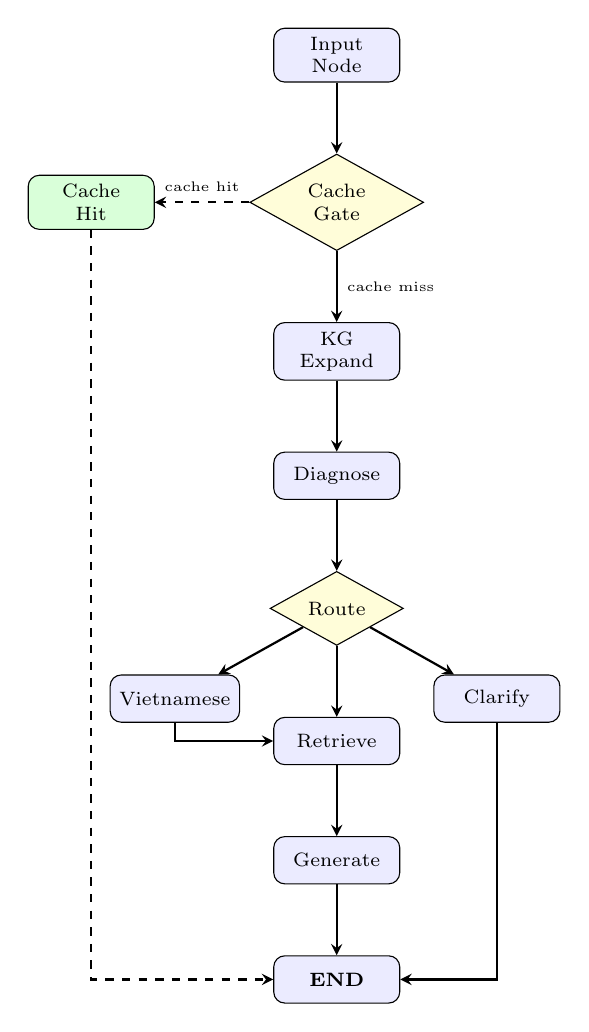
\begin{tikzpicture}[
  node distance=0.9cm and 0.6cm,
  block/.style={rectangle, draw, rounded corners, minimum width=1.6cm, minimum height=0.6cm, font=\scriptsize, align=center, fill=blue!8},
  decision/.style={diamond, draw, minimum width=1.2cm, minimum height=0.8cm, font=\scriptsize, align=center, fill=yellow!15, aspect=1.8},
  cache/.style={rectangle, draw, rounded corners, minimum width=1.6cm, minimum height=0.6cm, font=\scriptsize, align=center, fill=green!15},
  arr/.style={->, thick, >=stealth},
  arrfast/.style={->, thick, >=stealth, dashed},
]
  % Nodes
  \node[block] (input) {Input\\Node};
  \node[decision, below=of input] (cgate) {Cache\\Gate};
  \node[cache, left=1.2cm of cgate] (chit) {Cache\\Hit};

  \node[block, below=of cgate] (kg) {KG\\Expand};
  \node[block, below=of kg] (diag) {Diagnose};

  \node[decision, below=of diag] (route) {Route};
  
  \node[block, below left=0.6cm and 0.8cm of route] (viet) {Vietnamese};
  \node[block, below=of route] (retr) {Retrieve};
  \node[block, below right=0.6cm and 0.8cm of route] (clarify) {Clarify};
  
  \node[block, below=of retr] (gen) {Generate};
  \node[block, below=of gen] (end) {\textbf{END}};
  
  % Edges
  \draw[arr] (input) -- (cgate);
  \draw[arrfast] (cgate) -- node[above, font=\tiny] {cache hit} (chit);
  \draw[arrfast] (chit) |- (end);
  \draw[arr] (cgate) -- node[right, font=\tiny] {cache miss} (kg);
  \draw[arr] (kg) -- (diag);
  \draw[arr] (diag) -- (route);
  \draw[arr] (route) -- (viet);
  \draw[arr] (route) -- (retr);
  \draw[arr] (route) -- (clarify);
  \draw[arr] (viet) |- (retr);
  \draw[arr] (clarify) |- (end);
  \draw[arr] (retr) -- (gen);
  \draw[arr] (gen) -- (end);
\end{tikzpicture}
\caption{\graphcag{} StateGraph topology. Dashed edges indicate the Fast Path after a cache hit, while solid edges indicate the Slow Path entered on a cache miss and continuing through the full pipeline. The reference implementation runs KG expansion then diagnosis sequentially; optional routing nodes (e.g., domain-specific adapter branches or clarification paths) may be enabled depending on profile state and confidence.}
\label{fig:topology}
\end{figure}

\subsection{Execution Paths}

\graphcag{} defines two primary execution paths. Background jobs may be used for non-blocking updates but are not required for the core response path.

\subsubsection{Fast Path (Cache Hit)}
When the cache gate identifies a valid cached response for the normalized query-profile pair, the pipeline short-circuits directly to the response formatter. In the current microbenchmark, hit-path latency ranges from roughly \textbf{12ms to 21ms mean} across workloads with an in-process cache backend.

\subsubsection{Slow Path (Full Pipeline)}
On cache miss, the full pipeline executes: knowledge graph expansion, diagnosis, hybrid retrieval, and grounded generation. In the current deterministic benchmark, miss-path latency ranges from roughly \textbf{110ms to 183ms mean} depending on workload; LLM-backed deployments can be substantially slower.

\subsubsection{KV-Cache Augmented Generation (Proposed)}
When the active context contains a stable prefix (e.g., profile tier, policy template, and a recurring concept bundle), \graphcag{} can optionally use a CAG-style KV-cache augmentation for the local LLM: prefill a reusable prefix once, then reuse or patch the KV objects across similar turns under PCC-based risk gating (Section~\ref{sec:kvcache}). This optimization is designed to reduce \emph{prefill} cost and shift compute toward decode-only generation for recurring interaction patterns.

\subsubsection{Optional Background Jobs}
After responding, optional background jobs can update the knowledge graph with newly discovered patterns, generate supplemental artifacts, or update profile summaries. These jobs are \emph{non-blocking} and do not affect response latency.

\subsection{State Schema}

The pipeline state $\mathcal{S}$ is a typed dictionary with the following field groups:

\begin{equation}
\begin{aligned}
\mathcal{S} ={}& \langle \mathcal{S}_\text{input}, \mathcal{S}_\text{profile}, \mathcal{S}_\text{kg}, \mathcal{S}_\text{diag}, \\
& \mathcal{S}_\text{retr}, \mathcal{S}_\text{gen}, \mathcal{S}_\text{meta} \rangle
\end{aligned}
\end{equation}

\noindent where:
\begin{itemize}[leftmargin=*]
  \item $\mathcal{S}_\text{input}$: User input text, session ID, input type (text/voice).
  \item $\mathcal{S}_\text{profile}$: profile tier, error history, vocabulary count.
  \item $\mathcal{S}_\text{kg}$: Seed concepts, expanded nodes, traversal paths.
  \item $\mathcal{S}_\text{diag}$: Detected errors, root causes, confidence score.
  \item $\mathcal{S}_\text{retr}$: Vector hits, KG context, evidence bundle.
  \item $\mathcal{S}_\text{gen}$: final response, execution strategy, scores.
  \item $\mathcal{S}_\text{meta}$: Models used (accumulator), latency, cache status.
\end{itemize}

A key design feature is the \texttt{models\_used} field, which uses an \emph{accumulator pattern}: each node appends its model identifiers to the list, enabling end-to-end traceability without node coupling.

% ═══════════════════════════════════════════════════════════════════════════════
% 4. CORE ALGORITHMS
% ═══════════════════════════════════════════════════════════════════════════════
\section{Core Algorithms}
\label{sec:algorithms}

\subsection{Profile Cache Correctness and Risk-Aware Gating (\rapid{})}

Standard response caches treat a cache hit as a purely syntactic or semantic match (e.g., keying by normalized query). In profile-conditioned systems, however, reusing a prior response can be incorrect even when it is factually correct: the active user's intent, profile tier, task state, or progress may have changed.

\textbf{Profile Cache Correctness (PCC).} We say a cached entry $\langle F, P_c, R, \mathcal{B}, \sigma, t_c\rangle$ (fingerprint, profile context at creation, response, evidence bundle, execution plan, timestamp) is \emph{PCC-valid} for a new query-profile pair $(q, P)$ if all constraints hold:
\begin{enumerate}[leftmargin=*]
  \item \textbf{Intent-consistent}: $I(q, P)$ matches cached intent $I_c$.
  \item \textbf{Concept-consistent}: root-cause concept set drift is small: $\Delta_C = 1 - \text{Jaccard}(C, C_c) \leq \epsilon_C$.
  \item \textbf{Level-safe}: $|\ell - \ell_c| \leq 1$ (or a stricter policy).
  \item \textbf{Progress-safe}: profile progress drift $\Delta_{\text{prog}}$ is below a threshold.
  \item \textbf{Fresh}: staleness $s = (\text{now} - t_c)/\text{TTL}$ is acceptable.
\end{enumerate}

\textbf{Reuse Risk.} We combine these factors into a scalar reuse risk $\rho \in [0,1]$:
\begin{equation}
\label{eq:reuse_risk}
\begin{aligned}
\rho ={}& \text{clip}_{[0,1]}\Big( w_1\,\Delta_I + w_2\,\Delta_C + w_3\,\Delta_\ell \\
& + w_4\,\Delta_{\text{prog}} + w_5\,s \Big)
\end{aligned}
\end{equation}
where $\Delta_I$ is intent mismatch (0/1), $\Delta_\ell$ is normalized level drift, and $w_i$ are tunable weights.

\subsubsection{Risk-Aware Cache Gate}

The cache gate is the first decision point after a \emph{cheap fingerprint extraction} step. It determines whether a cached response can be reused, reused with a low-cost patch, or rejected (full pipeline).

\begin{algorithm}[h]
\caption{\rapid{} Risk-Aware Cache Gate with Delta Patching}
\label{alg:cache_gate}
\footnotesize
\begin{algorithmic}[1]
\REQUIRE Query $q$, Profile State $P$, Session Summary $S$, Cache Store $\mathcal{C}$
\ENSURE Decision $d \in \{\text{reuse},\text{patch},\text{full}\}$, Output $R$
\STATE $F \leftarrow \text{Fingerprint}(q, P, S)$ \COMMENT{intent, level, root-cause concepts, short history}
\STATE $k \leftarrow \text{Key}(F)$ \COMMENT{concept-level keying, versioned}
\STATE $e \leftarrow \mathcal{C}.\text{get}(k)$
\IF{$e = \text{null}$}
  \RETURN $(\text{full}, \text{null})$
\ENDIF
\STATE $\rho \leftarrow \text{ReuseRisk}(F, e)$ \COMMENT{Eq.~\ref{eq:reuse_risk}}
\IF{$\rho \leq \tau_0$ \AND \text{PCCValid}$(F,e)$}
  \RETURN $(\text{reuse}, e.R)$
\ELSIF{$\rho \leq \tau_1$ \AND \text{PCCPatchable}$(F,e)$}
  \STATE $R \leftarrow \text{Patch}(e.R, e.\sigma, P)$ \COMMENT{delta patch, no heavy retrieval}
  \RETURN $(\text{patch}, R)$
\ELSE
  \RETURN $(\text{full}, \text{null})$
\ENDIF
\end{algorithmic}
\end{algorithm}

\paragraph{Delta Caches.} Unlike response-only caching, we cache structured artifacts to enable low-cost patching:
\begin{itemize}[leftmargin=*]
  \item \textbf{Response cache} $\mathcal{C}_{\text{resp}}$: $R$ and correction metadata.
  \item \textbf{Evidence cache} $\mathcal{C}_{\text{ev}}$: evidence bundle $\mathcal{B}$ (KG snippets, examples).
  \item \textbf{Plan cache} $\mathcal{C}_{\text{plan}}$: execution plan $\sigma$ (strategy, difficulty, slot template).
\end{itemize}
These caches increase safe hit rates under PCC constraints and reduce generation cost via patching.

\subsubsection{Calibrated Reuse Verification and Action Selection}

The main theoretical weakness of a threshold-only gate is that $\tau_0$ and $\tau_1$ are heuristic unless tied to an explicit risk budget. We therefore refine \rapid{} as a \emph{calibrated decision rule}: reuse is permitted only when the estimated reuse risk is low \emph{and} the current state falls inside a confidence-controlled acceptance region.

Let $x$ denote the current decision state, including drift and systems features:
\begin{equation}
\label{eq:decision_state}
x = \langle \Delta_I, \Delta_C, \Delta_\ell, \Delta_{\text{prog}}, s, c, m, b \rangle
\end{equation}
where $c$ is diagnosis confidence, $m$ is memory pressure, and $b$ is the remaining latency budget. We define a nonconformity score
\begin{equation}
\label{eq:nonconformity}
\nu(x) = \rho(x) + \lambda_u (1-c) + \lambda_m m
\end{equation}
which augments reuse risk with uncertainty and systems pressure. Given a calibration set $\mathcal{D}_{\text{cal}}$ of historical decisions labeled by whether reuse preserved correctness, we compute the conformal quantile
\begin{equation}
\label{eq:conformal_quantile}
q_{1-\alpha} = \text{Quantile}_{1-\alpha}\big(\{\nu(x_i) : x_i \in \mathcal{D}_{\text{cal}}\}\big)
\end{equation}
for a target violation rate $\alpha$. The resulting acceptance region is
\begin{equation}
\label{eq:accept_region}
\mathcal{A}_{\alpha} = \{x : \nu(x) \leq q_{1-\alpha}\}
\end{equation}
so that reuse or patching is attempted only if $x \in \mathcal{A}_{\alpha}$. Intuitively, this turns PCC into a risk budget: smaller $\alpha$ yields a more conservative policy.

Within the acceptance region, the remaining choice is \emph{which} action to take. We define an action set
\begin{equation}
\label{eq:action_set}
\mathcal{U} = \{\text{reuse},\text{patch},\text{graph},\text{hybrid},\text{recompute}\}
\end{equation}
and score each action under a utility objective
\begin{equation}
\label{eq:utility_objective}
\begin{aligned}
J(a \mid x) ={}& \mathbb{E}\big[Q(a, x) - \beta_L L(a, x) - \beta_M M(a, x) \\
& - \beta_V V(a, x)\big]
\end{aligned}
\end{equation}
where $Q$ is correctness preservation, $L$ latency, $M$ memory cost, and $V$ a safety-violation penalty. The controller selects
\begin{equation}
\label{eq:action_argmax}
a^*(x) = \arg\max_{a \in \mathcal{U}} J(a \mid x)
\end{equation}
subject to the conformal guard in Eq.~\ref{eq:accept_region}. In practice, this objective can be realized with a lightweight contextual bandit or with offline threshold tuning; the important theoretical point is that reuse, patching, and retrieval become solutions to a common constrained optimization problem rather than separate heuristics.

This formulation sharpens the distinction between \graphcag{} and prior graph- or cache-centric systems. Graph retrieval is no longer the default front-end, and cache reuse is no longer an unconditional acceleration trick. Both become actions in a calibrated control policy over state drift.

\subsection{KV-Cache Augmentation (CAG-Style) for Profile-Conditioned Generation (Proposed)}
\label{sec:kvcache}

Response caching accelerates repeated queries, but misses still incur full prompt encoding and LLM inference. Inspired by CAG \cite{chan2024cag}, we propose a \emph{KV-cache augmentation} tier that pre-encodes stable profile-conditioned knowledge into the local LLM's \emph{past key-values} (KV cache) and reuses it across sessions.

\paragraph{Key challenge.} In profile-conditioned generation, the context is not fully static: profile tier, misconceptions, and session goals drift. Therefore, KV reuse must be \emph{conditioned} on PCC constraints and bounded by a strict safety policy.

\subsubsection{Tier-0 KV Cache Objects}

We define a reusable KV object as:
\begin{equation}
\label{eq:kv_object}
\mathcal{K} = \langle k_{\text{kv}},\; \text{prefix},\; \text{KV},\; \ell,\; C,\; t \rangle
\end{equation}
where \texttt{prefix} is a stable system+knowledge prompt (e.g., policy rules, concept summaries), \texttt{KV} are the cached transformer states, $\ell$ is profile tier, and $C$ is a concept bundle (e.g., a small community or root-cause set).

\paragraph{Indexing.} We propose indexing KV objects by a concept-level key:
\begin{equation}
k_{\text{kv}} = H\big(v \;\|\; \ell \;\|\; \text{ConceptBundle}(C)\big)
\end{equation}

\subsubsection{Warm-Up: Building KV Caches Offline or Background}

Warm-up can run at startup or asynchronously when traffic is low. The goal is to precompute \texttt{KV} for common (level, concept) bundles.

\begin{algorithm}[h]
\caption{WarmKVCache (Proposed)}
\label{alg:warm_kv}
\footnotesize
\begin{algorithmic}[1]
\REQUIRE KG $\mathcal{G}$, level set $\mathcal{L}$, warm bundles $\mathcal{B}$, local LLM $f_{\text{LLM}}$
\ENSURE KV store $\mathcal{C}_{\text{kv}}$
\FOR{each $(\ell, C) \in \mathcal{B}$}
  \STATE $\text{prefix} \leftarrow \text{BuildPrefix}(\ell, C, \mathcal{G})$ \COMMENT{persona + pedagogy + concept summaries}
  \STATE $\text{KV} \leftarrow f_{\text{LLM}}.\text{encode}(\text{prefix})$ \COMMENT{compute past\_key\_values}
  \STATE $k_{\text{kv}} \leftarrow H(v \;\|\; \ell \;\|\; \text{ConceptBundle}(C))$
  \STATE $\mathcal{C}_{\text{kv}}[k_{\text{kv}}] \leftarrow \langle k_{\text{kv}}, \text{prefix}, \text{KV}, \ell, C, \text{now}\rangle$
\ENDFOR
\RETURN $\mathcal{C}_{\text{kv}}$
\end{algorithmic}
\end{algorithm}

\subsubsection{Inference-Time Reuse with PCC Gating and Delta Patching}

At inference, we first attempt response-cache reuse (Tier 1). On miss, we attempt KV reuse (Tier 0) if PCC constraints allow it. If reuse risk is moderate, we apply a \emph{delta-prefix} patch (small, cheap) rather than rebuilding the full prefix.

\begin{algorithm}[h]
\caption{KVReuseOrRecompute (Proposed)}
\label{alg:kv_reuse}
\footnotesize
\begin{algorithmic}[1]
\REQUIRE Query $q$, profile state $P$, concept bundle $C$, KV store $\mathcal{C}_{\text{kv}}$, local LLM $f_{\text{LLM}}$
\ENSURE Past KV for generation, decision flag
\STATE $k_{\text{kv}} \leftarrow H(v \;\|\; P.\ell \;\|\; \text{ConceptBundle}(C))$
\STATE $\mathcal{K} \leftarrow \mathcal{C}_{\text{kv}}.\text{get}(k_{\text{kv}})$
\IF{$\mathcal{K}=\text{null}$}
  \RETURN $(\text{recompute},\; f_{\text{LLM}}.\text{encode}(\text{BuildPrefix}(P.\ell, C)))$
\ENDIF
\STATE $\rho \leftarrow \text{ReuseRisk}(\text{Fingerprint}(q,P,\cdot), \mathcal{K})$
\IF{$\rho \leq \tau_0$}
  \RETURN $(\text{reuse},\; \mathcal{K}.\text{KV})$
\ELSIF{$\rho \leq \tau_1$}
  \STATE $\delta \leftarrow \text{BuildDeltaPrefix}(P, q)$ \COMMENT{short profile/session patch}
  \STATE $\text{KV}' \leftarrow f_{\text{LLM}}.\text{encode}(\delta, \text{pastKV}=\mathcal{K}.\text{KV})$
  \RETURN $(\text{patch},\; \text{KV}')$
\ELSE
  \RETURN $(\text{recompute},\; f_{\text{LLM}}.\text{encode}(\text{BuildPrefix}(P.\ell, C)))$
\ENDIF
\end{algorithmic}
\end{algorithm}

\paragraph{Generation.} Given a selected past KV, the model decodes the tutor response by appending the user query (and optional evidence snippets) and running only the decoding steps:
\begin{equation}
\begin{aligned}
R \leftarrow{}& f_{\text{LLM}}.\text{decode}(q \;\|\|\; \mathcal{B}, \\
& \text{pastKV}=\text{KV})
\end{aligned}
\end{equation}

\paragraph{Safety note.} KV augmentation is only safe when the prefix is stable and when PCC constraints are satisfied. In the current reference implementation, KV augmentation is a planned extension; we include it here to define a concrete flow and evaluation target.

\subsection{Knowledge Graph Expansion}

The KG expansion algorithm performs a two-phase process: seed matching and BFS expansion.

\subsubsection{Phase 1: Seed Concept Matching}

Given user text $t$, we identify seed concepts $C_\text{seed}$ via two methods:

\begin{enumerate}[leftmargin=*]
  \item \textbf{Keyword matching}: For each concept $c \in \mathcal{G}$, check if any keyword $w \in c.\text{keywords}$ appears in $t$.
  \item \textbf{Pattern matching}: Apply regex patterns that map common error structures to grammar concepts (e.g., \texttt{/\textbackslash bi goes\textbackslash b/} $\rightarrow$ \texttt{subject\_verb\_agreement}).
\end{enumerate}

\begin{equation}
\begin{aligned}
C_\text{seed} ={}& \{c \in \mathcal{G} \mid \exists w \in c.\text{kw}: w \in t\} \\
& \cup \{c \mid \exists p \in \mathcal{P}: p.\text{regex} \sim t\}
\end{aligned}
\end{equation}

\subsubsection{Phase 2: Level-Aware Best-First Expansion}

From seed concepts, we perform a level-aware best-first expansion (priority search). This differs from strict BFS because neighbor expansion is prioritized by profile relevance (Eq.~\ref{eq:pedweight}).

\begin{algorithm}[h]
\caption{Level-Aware Best-First Graph Expansion}
\label{alg:bfs}
\footnotesize
\begin{algorithmic}[1]
\REQUIRE Seeds $C_\text{seed}$, KG $\mathcal{G}$, profile tier $\ell$, max hops $h$, max nodes $n$
\ENSURE Expanded nodes $E$, Paths $\Pi$
\STATE $Q \leftarrow \text{PriorityQueue}(C_\text{seed})$ \COMMENT{best-first frontier}
\STATE $E \leftarrow \emptyset$; $\Pi \leftarrow \emptyset$; $V \leftarrow C_\text{seed}$
\WHILE{$Q \neq \emptyset$ \AND $|E| < n$}
    \STATE $(c, d) \leftarrow Q.\text{dequeue}()$
    \IF{$d > h$}
        \STATE \textbf{continue}
    \ENDIF
    \FOR{\textbf{each} $(c, c', r) \in \mathcal{G}.\text{edges}(c)$}
        \IF{$c' \notin V$}
        \STATE $w \leftarrow \text{PedWeight}(r, \ell)$ \COMMENT{Eq.~\ref{eq:pedweight}}
            \STATE $Q.\text{push}((c', d+1), \text{priority}=w)$
            \STATE $V \leftarrow V \cup \{c'\}$
            \STATE $E \leftarrow E \cup \{(c', r, c'.\text{props})\}$
            \STATE $\Pi \leftarrow \Pi \cup \{(c \rightarrow c', r, d+1)\}$
        \ENDIF
    \ENDFOR
\ENDWHILE
\RETURN $(E, \Pi)$
\end{algorithmic}
\end{algorithm}

The profile-aware weight function prioritizes concepts relevant to the active profile tier:

\begin{equation}
\label{eq:pedweight}
  w(r, \ell) = \begin{cases}
    1.0 & \text{if } r.\text{level} = \ell \\
    0.7 & \text{if } |r.\text{level} - \ell| = 1 \\
    0.3 & \text{otherwise}
  \end{cases}
\end{equation}

\noindent where $\ell$ is the active CEFR-style profile tier mapped to numerical values (A1=1, A2=2, ..., C2=6).

\subsection{AI-Powered Diagnosis}

The diagnosis node performs comprehensive linguistic analysis through a structured LLM prompt:

\begin{equation}
\begin{aligned}
\mathcal{D}(t, \ell) ={}& f_\text{LLM}\big(\text{prompt}_\text{diag}(t, \ell)\big) \\
& \rightarrow \langle E, I, s_g, s_f, c \rangle
\end{aligned}
\end{equation}

\noindent where $E$ is the set of detected errors (each with span, type, correction, explanation), $I$ is the detected intent (correct$|$explain$|$practice$|$ask), $s_g$ is the grammar score, $s_f$ is the fluency score, and $c$ is the confidence.

A \textbf{rule-based fallback} activates when AI diagnosis fails or confidence $c < 0.5$:

\begin{equation}
\begin{aligned}
\mathcal{D}_\text{fallback}(t) ={}& \{(m, \tau, c_\tau, e_\tau) \\
& \mid \exists r \in \mathcal{R}: r.\text{regex} \sim t\}
\end{aligned}
\end{equation}

\noindent where $\mathcal{R}$ is a curated set of grammar rules with regex patterns, and $(m, \tau, c_\tau, e_\tau)$ are the matched span, error type, correction, and explanation respectively.

\subsection{Budgeted (Anytime) Hybrid Retrieval}

The retrieval node combines knowledge graph evidence with vector similarity search:

\begin{algorithm}[h]
\caption{Budgeted Hybrid Retrieval (Anytime)}
\label{alg:hybrid}
\footnotesize
\begin{algorithmic}[1]
\REQUIRE Diagnosis $\mathcal{D}$, KG nodes $E$, User text $t$, Embedding model $\phi$, Budget $B$
\ENSURE Evidence bundle $\mathcal{B}$
\STATE \COMMENT{--- Stage 1: Graph-local evidence (cheap) ---}
\STATE $\mathcal{B} \leftarrow \emptyset$
\STATE $\mathcal{B} \leftarrow \mathcal{B} \cup \text{BestFirst}(\mathcal{G}, \mathcal{D}.\text{root\_causes} \cup E, h{=}2, n{=}10, \text{budget}=B)$
\IF{\text{Sufficient}$(\mathcal{B})$ \OR $\text{BudgetExhausted}(B)$}
  \RETURN $\mathcal{B}$
\ENDIF
\STATE \COMMENT{--- Stage 2: Optional vector evidence (budgeted) ---}
\STATE $\mathbf{v} \leftarrow \phi(t)$
\STATE $E_\text{vec} \leftarrow \text{ANNIndex}.\text{search}(\mathbf{v}, k{=}5)$ \COMMENT{e.g., FAISS/HNSW}
\STATE $\mathcal{B} \leftarrow \mathcal{B} \cup E_\text{vec}$
\RETURN $\text{Top}_k(\mathcal{B}, k{=}5)$
\end{algorithmic}
\end{algorithm}

When both graph and vector candidates are available, we rank evidence using a lightweight fusion function (optional) to trade off structural proximity, semantic similarity, and recency in the active profile history.

\begin{equation}
\label{eq:fusion}
\text{score}(e) = \alpha \cdot s_\text{kg}(e) + \beta \cdot s_\text{vec}(e) + \gamma \cdot s_\text{rec}(e)
\end{equation}

\noindent where:
\begin{itemize}[leftmargin=*]
  \item $s_\text{kg}(e)$: Knowledge graph relevance (inverse hop distance from seed). $s_\text{kg}(e) = \frac{1}{1 + d(e)}$, where $d(e)$ is the BFS depth.
  \item $s_\text{vec}(e)$: Cosine similarity from vector search. $s_\text{vec}(e) = \cos(\mathbf{v}_q, \mathbf{v}_e)$.
  \item $s_\text{rec}(e)$: Recency bonus based on how recently the concept was taught. $s_\text{rec}(e) = \exp(-\lambda \cdot \Delta t)$, where $\Delta t$ is time since last usage.
  \item Weights: $\alpha = 0.5$, $\beta = 0.3$, $\gamma = 0.2$ (tunable).
\end{itemize}

\subsection{Conditional Routing}

After diagnosis, the pipeline routes to one of three sub-paths based on confidence and profile tier:

\begin{equation}
\text{Route}(\mathcal{S}) = \begin{cases}
  \text{ask\_clarify} & \text{if } c < 0.5 \\
  \text{vietnamese} \to \text{retrieve} & \text{if } \ell \in \{A1, A2\} \wedge |E| > 0 \\
  \text{retrieve} & \text{otherwise}
\end{cases}
\end{equation}

In the language-learning instantiation, the Vietnamese path generates native-language explanations for beginner users before proceeding to retrieval, following the \emph{L1 scaffolding} principle in second language acquisition theory.

\subsection{Grounded Generation}

The generation node constructs a context-enriched prompt from the evidence bundle, ensuring the LLM response is grounded in verified linguistic knowledge:

\begin{equation}
\begin{aligned}
R ={}& f_\text{LLM}\big(\text{persona} \;\|\; \mathcal{B}_\text{evidence} \\
& \;\|\; \text{history} \;\|\; q\big)
\end{aligned}
\end{equation}

The execution strategy is determined by error count and fluency:

\begin{equation}
\label{eq:strategy}
\sigma = \begin{cases}
  \text{PRAISE} & \text{if } |E| = 0 \\
  \text{FEEDBACK} & \text{if } 1 \leq |E| \leq 2 \\
  \text{SCAFFOLD} & \text{if } |E| > 2 \\
  \text{SOCRATIC} & \text{if } I = \text{explain} \wedge s_f > 0.7
\end{cases}
\end{equation}

% ═══════════════════════════════════════════════════════════════════════════════
% 5. MEMORY MANAGEMENT
% ═══════════════════════════════════════════════════════════════════════════════
\section{Memory-Aware Model Management}
\label{sec:memory}

A critical challenge in \graphcag{} is managing 5+ AI models within a constrained memory budget. We formalize this as a \textbf{model scheduling problem}.

\subsection{Problem Formulation}

Let $\mathcal{M} = \{m_1, m_2, \ldots, m_n\}$ be the set of registered models, each with:
\begin{itemize}[leftmargin=*]
  \item $\text{mem}(m_i)$: Memory footprint in MB.
  \item $\text{pri}(m_i) \in \{\text{CRITICAL},\text{HIGH},\text{NORMAL},\text{LOW}\}$: Priority class.
  \item $\text{idle}(m_i)$: Time since last invocation.
  \item $\tau(m_i)$: Idle timeout threshold.
\end{itemize}

We define an eviction rank function $\text{PriRank}(\cdot)$ such that:

\begin{equation}
\text{PriRank}(\text{LOW}) > \text{PriRank}(\text{NORMAL}) > \text{PriRank}(\text{HIGH}) > \text{PriRank}(\text{CRITICAL})
\end{equation}

\noindent Only non-critical models are evictable.

The total memory constraint is:
\begin{equation}
\sum_{m_i \in \mathcal{M}_\text{loaded}} \text{mem}(m_i) \leq M_\text{max}
\end{equation}

\subsection{Model Registry}

Table~\ref{tab:models} shows the model registry for the reference instantiation with memory and priority configurations:

\begin{table}[h]
\centering
\caption{Model registry with memory and scheduling parameters.}
\label{tab:models}
{\scriptsize
\setlength{\tabcolsep}{4pt}
\resizebox{\columnwidth}{!}{%
\begin{tabular}{@{}lcccr@{}}
\toprule
\textbf{Model} & \textbf{Type} & \textbf{Mem} & \textbf{Pri} & \textbf{Idle} \\
\midrule
Qwen2.5-1.5B  & chat       & 1,600MB & CRITICAL & $\infty$ \\
Whisper-v3     & stt        & 244MB   & NORMAL   & 300s \\
MiniLM-L6-v2  & embedding  & 22MB    & HIGH     & 600s \\
HuBERT-large  & pronun.    & 960MB   & LOW      & 60s \\
Piper-VITS    & tts        & 60MB    & NORMAL   & 300s \\
\bottomrule
\end{tabular}
}
}
\end{table}

\subsection{Lazy Loading with Priority Eviction}

When a model $m_j$ is requested but not loaded, the gateway must ensure sufficient memory:

\begin{algorithm}[h]
\caption{Memory-Aware Model Loading}
\label{alg:memory}
\footnotesize
\begin{algorithmic}[1]
\REQUIRE Model $m_j$ to load, Budget $M_\text{max}$
\ENSURE $m_j$ is loaded and ready
\STATE $M_\text{avail} \leftarrow M_\text{max} - \sum_{m_i \in \mathcal{M}_\text{loaded}} \text{mem}(m_i)$
\IF{$\text{mem}(m_j) \leq M_\text{avail}$}
    \STATE $\text{Load}(m_j)$ \COMMENT{Sufficient memory}
\ELSE
    \STATE \COMMENT{Evict lowest-priority idle models}
  \STATE $\mathcal{E} \leftarrow \text{sort}(\mathcal{M}_\text{loaded}, \text{key}=(\text{PriRank} \downarrow, \text{idle} \downarrow))$
    \WHILE{$M_\text{avail} < \text{mem}(m_j)$ \AND $\mathcal{E} \neq \emptyset$}
        \STATE $m_e \leftarrow \mathcal{E}.\text{pop}()$
        \IF{$\text{pri}(m_e) \neq \text{CRITICAL}$}
            \STATE $\text{Unload}(m_e)$
            \STATE $M_\text{avail} \leftarrow M_\text{avail} + \text{mem}(m_e)$
        \ENDIF
    \ENDWHILE
    \IF{$M_\text{avail} \geq \text{mem}(m_j)$}
        \STATE $\text{Load}(m_j)$
    \ELSE
        \STATE \textbf{raise} MemoryError
    \ENDIF
\ENDIF
\end{algorithmic}
\end{algorithm}

\subsection{Auto-Unload Policy}

A background task periodically checks for idle models:

\begin{equation}
\text{Evict}(m_i) \iff \text{idle}(m_i) > \tau(m_i) \wedge \text{pri}(m_i) \neq \text{CRITICAL}
\end{equation}

This ensures that the Qwen chat model (CRITICAL) remains loaded at all times while memory-heavy models like HuBERT (960MB, LOW priority) are unloaded after 60 seconds of idle time.

\subsection{Memory Budget Analysis}

Memory footprints vary significantly by model variant, quantization, runtime (CPU vs GPU), and batch configuration. Therefore, we treat model memory as a configuration-dependent parameter obtained from the model registry.

Let $\text{mem}(m)$ denote the measured or estimated footprint for model $m$ in the current deployment. Worst-case and typical footprints are summarized as:
\begin{equation}
\begin{aligned}
M_{\text{worst}} ={}& \sum_{m \in \mathcal{M}} \text{mem}(m), \\
M_{\text{typical}} ={}& \sum_{m \in \mathcal{M}_{\text{hot}}} \text{mem}(m)
\end{aligned}
\end{equation}
where $\mathcal{M}_{\text{hot}}$ is the set of frequently used models kept warm (e.g., chat + embedding + STT). The gateway enforces $\sum_{m \in \mathcal{M}_{\text{loaded}}} \text{mem}(m) \le M_{\max}$ via priority eviction (Alg.~\ref{alg:memory}).

\paragraph{KV-cache objects (proposed).} If KV-cache augmentation (Section~\ref{sec:kvcache}) is enabled, the system must also budget for cached \emph{past key-values}. Let $\mathcal{K}_{\text{loaded}}$ be the set of resident KV objects and $\text{mem}(\mathcal{K}_j)$ their measured footprint. Then:
\begin{equation}
\begin{aligned}
& \sum_{m \in \mathcal{M}_{\text{loaded}}} \text{mem}(m) \\
& + \sum_{\mathcal{K}_j \in \mathcal{K}_{\text{loaded}}} \text{mem}(\mathcal{K}_j) \le M_{\max}
\end{aligned}
\end{equation}

We propose a simple eviction rule that mirrors model eviction: evict lowest-priority, least-recently-used KV objects when memory pressure is detected. Priority can be derived from profile-tier frequency and concept bundle popularity.

% ═══════════════════════════════════════════════════════════════════════════════
% 6. CACHING STRATEGY
% ═══════════════════════════════════════════════════════════════════════════════
\section{Multi-Level Caching Strategy}
\label{sec:caching}

\graphcag{} employs response caching to enable a Fast Path on repeated interaction patterns. In the reference implementation, Redis is an \emph{optional} backend; if unavailable, the system falls back to an in-process TTL cache. \rapid{} extends this with concept-level fingerprints and \emph{delta caches} (evidence and plan artifacts) to enable low-cost patching.

\subsection{Tier 0: KV Cache Augmentation (\rapid{}, proposed)}

When using a local LLM backend, we propose an additional cache tier that stores \emph{past key-values} for stable profile-conditioned prefixes (Section~\ref{sec:kvcache}). Concept-level indexing and PCC gating are required to keep reuse safe.

This tier targets reductions in \emph{prefill} cost on slow-path misses by reusing pre-encoded instruction + knowledge prefixes, while still allowing query-specific decoding.

\subsection{Tier 1: Response Cache}

\paragraph{Reference key (implemented).} In the current reference implementation, we use a simple response key to prioritize robustness and low overhead:

\begin{equation}
\label{eq:cache_key_ref}
k_{\text{ref}} = \text{MD5}\big(\text{clean}(q) \;\|\|\; \ell\big)
\end{equation}

\noindent where $\ell$ is the active CEFR-style profile tier. This key supports high hit rates for identical or case/trim-normalized repeated queries but does not encode PCC constraints and is brittle to prompt wrappers or small formatting changes.

\paragraph{\rapid{} key (proposed).} \rapid{} generalizes the key to a concept-level fingerprint:

\begin{equation}
\label{eq:cache_key}
k = H\big(v \;\|\; \text{Fingerprint}(q, P, S)\big)
\end{equation}

\noindent where $H$ is a hash function (e.g., MD5/SHA-256) and the fingerprint is concept-level rather than text-only (intent, CEFR level, root-cause concept set, and a short session summary).

\begin{equation}
\begin{aligned}
\mathcal{C}_\text{resp}[k] ={}& \langle R, \text{corrections}, \text{scores}, \\
& \text{strategy}, t_\text{created} \rangle
\end{aligned}
\end{equation}

\noindent Controlled repeated-query benchmarks reach a 50.0\% hit rate by construction, but this should be interpreted as a stress test of exact-repeat reuse rather than a deployment prior. In the same benchmark, prompt wrappers, punctuation edits, and internal whitespace perturbations fall through to the Slow Path, which confirms that the present implementation is still a lower-bound approximation of the PCC design.

\subsection{Tier 2: Evidence and Plan Delta Caches (\rapid{}, proposed)}

We cache structured artifacts that allow patching when reuse risk is moderate:
\begin{equation}
\begin{aligned}
\mathcal{C}_\text{ev}[k] ={}& \langle \mathcal{B}, t_\text{created} \rangle, \\
\mathcal{C}_\text{plan}[k] ={}& \langle \sigma, t_\text{created} \rangle
\end{aligned}
\end{equation}

These caches reduce repeated retrieval and enable low-cost regeneration (e.g., adjusting difficulty or examples) without re-running the entire pipeline.

\subsection{Tier 3: TTS Audio Cache (optional)}

Text-to-speech outputs are expensive to regenerate. We cache using MD5 of the cleaned text:

\begin{equation}
\begin{aligned}
\mathcal{C}_\text{tts}[\text{MD5}(\text{clean}(R))] ={}& \langle \text{audio\_b64}, \\
& \text{duration}, t_\text{created} \rangle
\end{aligned}
\end{equation}

\noindent TTL: 7 days. This cache is typically implemented at the caller/client layer (since TTS may be handled outside the core \graphcag{} graph).

\subsection{Tier 4: Profile Cache (optional)}

Profile records are cached to avoid database lookups:

\begin{equation}
\mathcal{C}_\text{profile}[\text{user\_id}] = \langle P, \text{error\_history}, \text{session\_count} \rangle
\end{equation}

\noindent TTL: 24 hours. Invalidated on profile update.

\subsection{Tier 5: KG Expansion Cache (optional)}

Knowledge graph expansion results for common concept combinations:

\begin{equation}
\begin{aligned}
\mathcal{C}_\text{kg}[\text{hash}(C_\text{seed})] ={}& \langle E_\text{expanded}, \\
& \Pi_\text{paths}, t_\text{created} \rangle
\end{aligned}
\end{equation}

\noindent TTL: 1 hour (KG structure is relatively static).

\subsection{Cache Versioning}

Following GraphRAG's approach \cite{edge2024graphrag}, we maintain a cache version counter:

\begin{equation}
\text{CACHE\_VERSION} = 1
\end{equation}

\noindent Keys include the version prefix: \texttt{v\{VERSION\}:resp:}\allowbreak\texttt{\{hash\}}. On schema changes, incrementing the version effectively invalidates all stale entries without explicit deletion.

% ═══════════════════════════════════════════════════════════════════════════════
% 7. IMPLEMENTATION
% ═══════════════════════════════════════════════════════════════════════════════
\section{Reference Framework Instantiation}
\label{sec:implementation}

\subsection{Reference Stack}

\begin{table}[h]
\centering
\caption{Technology stack for the open reference instantiation used in the microbenchmark.}
\label{tab:stack}
{\scriptsize
\setlength{\tabcolsep}{4pt}
\begin{tabularx}{\columnwidth}{@{}Y Y@{}}
\toprule
\textbf{Component}      & \textbf{Technology} \\
\midrule
Pipeline Engine          & LangGraph StateGraph \\
Knowledge Graph          & KuzuDB (embedded graph DB) \\
Vector Retrieval          & MiniLM similarity over KG-derived candidate labels (no vector DB required) \\
Vector Store (optional)  & FAISS/HNSW (not required for the reference implementation) \\
Embedding Model          & all-MiniLM-L6-v2 (22MB) \cite{wang2020minilm,reimers2019sentencebert} \\
Chat LLM (local)         & Qwen2.5-1.5B-Instruct + LoRA \\
Chat LLM (cloud)         & Groq (LLaMA-3.3-70B) / Gemini 2.0 \\
STT                      & Whisper-v3 \\
TTS                      & gTTS (external) / Piper VITS (optional) \\
Cache                    & Redis 7.x (optional) + in-process TTL fallback \\
API Framework            & FastAPI (Python 3.11) \\
\bottomrule
\end{tabularx}
}
\end{table}

\subsection{LangGraph StateGraph Construction}

We present a reference StateGraph construction used to instantiate \graphcag{}. Optional routing nodes (e.g., domain adapters or clarification prompts on low confidence) are included for completeness.

The graph is constructed declaratively:

\begin{lstlisting}[caption={StateGraph construction in Python.},label={lst:graph}]
graph = StateGraph(GraphCAGState)

# Nodes
graph.add_node("input_node", input_node)
graph.add_node("cache_gate_node", cache_gate_node)
graph.add_node("kg_expand_node", kg_expand_node)
graph.add_node("diagnose_node", diagnose_node)
graph.add_node("retrieve_node", retrieve_node)
graph.add_node("generate_node", generate_node)
graph.add_node("vietnamese_node", vietnamese_node)      # optional
graph.add_node("ask_clarify_node", ask_clarify_node)    # optional
graph.add_node("tts_node", tts_node)                    # optional

# Entry + Cache Gate
graph.set_entry_point("input_node")
graph.add_edge("input_node", "cache_gate_node")
graph.add_conditional_edges(
  "cache_gate_node", check_cache_hit,
  {"cache_hit": END, "process": "kg_expand_node"})

# Sequential slow path
graph.add_edge("kg_expand_node", "diagnose_node")

# Conditional: diagnose -> retrieve | vietnamese | ask_clarify
graph.add_conditional_edges(
  "diagnose_node", route_after_diagnosis,
  {"retrieve_node": "retrieve_node",
   "vietnamese_node": "vietnamese_node",
   "ask_clarify_node": "ask_clarify_node"})

# Vietnamese -> retrieve
graph.add_edge("vietnamese_node", "retrieve_node")

# Route + Generate
graph.add_edge("retrieve_node", "generate_node")
graph.add_edge("ask_clarify_node", END)

# Optional: generate -> tts -> end
graph.add_conditional_edges(
  "generate_node", should_generate_tts,
  {"tts_node": "tts_node", "end": END})
graph.add_edge("tts_node", END)
\end{lstlisting}

\subsection{LLM Fallback Chain}

The system employs a three-tier LLM fallback for resilience:

\begin{enumerate}[leftmargin=*]
  \item \textbf{Groq API} (e.g., LLaMA-3.x class): Primary for production.
  \item \textbf{Gemini API} (Gemini-class): Cloud fallback.
  \item \textbf{Ollama} (Qwen2.5-1.5B + LoRA): Offline fallback.
\end{enumerate}

Observed latency depends on network, model choice, and prompt size; we report end-to-end profiling targets and microbenchmarks separately.

\subsection{From Prototype to Full \rapid{}}

The algorithms in Sections~\ref{sec:algorithms} and \ref{sec:caching} describe the \emph{full target realization} of \rapid{}, not merely the currently benchmarked subset. This is important for interpretation: the paper's primary technical object is the full graph-and-cache control policy, while the present implementation should be read as an executable lower bound that already validates the graph skeleton, the cache short-circuit, and the surrounding retrieval pipeline.

The key reason this target design remains practically feasible is that it can be realized through \emph{incremental substitutions} inside an already working graph rather than through a full architectural rewrite. Concretely, the current prototype already has (i) a dedicated cache-gate node, (ii) a stable Slow Path for graph expansion, diagnosis, retrieval, and generation, and (iii) persistent cache backends with versioned keys. Full \rapid{} therefore requires replacing local decision rules and cache payloads, not replacing the overall StateGraph.

We view the realization path as four engineering stages:
\begin{enumerate}[leftmargin=*]
  \item \textbf{Stage 1: executable lower bound (current).} Response reuse is keyed by normalized query text plus learner level, giving a conservative fast path that is easy to validate and easy to disable when unsafe.
  \item \textbf{Stage 2: structured cache entries.} The response cache is upgraded to store profile snapshots, concept sets, evidence bundles, and execution plans alongside the final response, enabling PCC checks on richer state than text alone.
  \item \textbf{Stage 3: risk-gated patching.} The binary reuse-or-full decision is replaced by a ternary controller (reuse, patch, full), with a dedicated patch path that reuses evidence and plan artifacts when drift is moderate but not negligible.
  \item \textbf{Stage 4: KV-cache augmentation.} Stable profile-conditioned prefixes are pre-encoded for the local LLM so that even Slow Path misses can avoid repeated prefill when the pedagogical prefix remains valid.
\end{enumerate}

This staged path explains why the full \rapid{} specification is not an unrealistic add-on. Each stage refines a component that already exists in the reference system: the cache gate becomes richer, cache entries become more structured, the routing graph gains a patch branch, and the local model backend gains a reusable KV tier. Because these refinements are modular, the paper can describe the full target design now while still grounding its feasibility in a working prototype and measurable intermediate milestones.

\subsection{KV-Cache Integration Notes (Proposed)}
The KV-cache augmentation in Section~\ref{sec:kvcache} is designed to be implementable in the local inference backend (e.g., Transformers/Ollama-hosted Qwen). Concretely, the system would (i) define a small set of canonical prefixes $\pi$ (profile tier + policy template + concept bundle), (ii) prefill the LLM once to obtain \texttt{past\_key\_values} for each $\pi$, and (iii) reuse or patch these KV objects at inference time when PCC-based gating deems reuse safe.

In practice, integration requires: (a) storing KV objects in an in-memory store with an explicit byte budget and eviction policy (Section~\ref{sec:memory}), (b) ensuring tokenizer/prompt canonicalization is stable so that KV reuse aligns to token boundaries, and (c) falling back to a full prefill when the selected prefix is unsafe (high reuse risk), drifted (prefix mismatch), or missing.

\subsection{LoRA Fine-Tuning Configuration}

The Qwen base model is fine-tuned with a unified LoRA adapter for multi-task performance:

\begin{equation}
\begin{aligned}
W' ={}& W + \Delta W = W + BA, \\
& B \in \mathbb{R}^{d \times r},\; A \in \mathbb{R}^{r \times d}
\end{aligned}
\end{equation}

\noindent Configuration: $r=48$, $\alpha=96$, dropout$=0.05$, targeting 7 modules (\texttt{q\_proj}, \texttt{k\_proj}, \texttt{v\_proj}, \texttt{o\_proj}, \texttt{gate\_proj}, \texttt{up\_proj}, \texttt{down\_proj}), yielding $\sim$45M trainable parameters ($\sim$80MB adapter file).

% ═══════════════════════════════════════════════════════════════════════════════
% 8. EXPERIMENTS
% ═══════════════════════════════════════════════════════════════════════════════
\section{Experimental Setup and Microbenchmarks}
\label{sec:experiments}

We report a reproducible microbenchmark that isolates \graphcag{}'s \emph{pipeline overhead} and cache effectiveness without relying on external LLM endpoints.

Unless otherwise stated, the experiments in this section evaluate the \emph{Stage 1 executable lower bound} described in Section~\ref{sec:implementation}; they should therefore be read as feasibility evidence for the full \rapid{} design rather than as an end-to-end measurement of every proposed component.

\subsection{Task and Dataset}

We sample English learner text from the Wi+Locness corpus (development split) in JSONL format. Each sample is treated as a short-form grounded correction request, which serves as a concrete profile-conditioned workload rather than the definition of the framework's entire scope.

\subsection{Benchmark Protocol}

We run an open-source benchmark harness released with the artifact using 20 unique samples per workload, each repeated twice under a fixed B1 learner profile, yielding 40 total runs per workload. The harness supports both single-text correction inputs and chat-style examples, allowing us to benchmark both correction and dialogue-style workloads. To reduce variance and avoid outbound calls, we fix:
\begin{itemize}[leftmargin=*]
  \item \texttt{diagnosis\_policy=rules}: deterministic rule-based diagnosis.
  \item \texttt{generation\_policy=template}: deterministic template generation.
\end{itemize}

We compare two modes:
\begin{itemize}[leftmargin=*]
  \item \textbf{LightRAG-style baseline}: cache disabled with full retrieval on every request.
  \item \textbf{\rapid{} mode}: response cache enabled with the budgeted retrieval policy used by the reference prototype.
\end{itemize}

\paragraph{Cache backend.} During the reported run, Redis was unavailable, so the reference implementation fell back to an in-process TTL cache. The reported hit-rate therefore reflects repeated queries within the same process rather than a distributed cache deployment.

\subsection{Results}

Table~\ref{tab:microbench} summarizes the primary Wi+Locness-derived benchmark used throughout the paper. Table~\ref{tab:multibench} then broadens the evaluation to additional workloads drawn from a held-out mixed-task validation corpus, and Table~\ref{tab:feasibility} reports the practical selectivity checks that matter most for feasibility claims.

\begin{table}[h]
\centering
\caption{Measured microbenchmark results (40 runs, B1, rule diagnosis + template generation).}
\label{tab:microbench}
{\scriptsize
\setlength{\tabcolsep}{3pt}
\resizebox{\columnwidth}{!}{%
\begin{tabular}{@{}lccccr@{}}
\toprule
\textbf{Mode} & \textbf{HitRate} & \textbf{Mean (ms)} & \textbf{P50 (ms)} & \textbf{P95 (ms)} & \textbf{HitMean (ms)} \\
\midrule
LightRAG (no-cache, full)     & 0.0\%  & 177.3 & 170.0 & 278.5 & -- \\
\rapid{} (cache, rapid)      & 50.0\% & 100.1 & 74.5 & 219.6 & 16.7 \\
\bottomrule
\end{tabular}
}
}
\end{table}

These results demonstrate that repeated-query reuse can reduce average latency substantially when exact-match patterns occur. Relative to the LightRAG-style baseline, the current \rapid{} prototype reduces mean latency by approximately 43.5\% (177.3ms $\rightarrow$ 100.1ms) while preserving a similar miss-path cost (183.5ms mean miss latency in the run log), indicating that the observed gain comes from actual fast-path reuse rather than an artificially weakened Slow Path.

\begin{table}[h]
\centering
\caption{Cross-workload efficiency benchmark with repeated-query evaluation (40 runs per workload).}
\label{tab:multibench}
{\scriptsize
\setlength{\tabcolsep}{3pt}
\resizebox{\columnwidth}{!}{%
\begin{tabular}{@{}llccccc@{}}
\toprule
\textbf{Workload} & \textbf{Mode} & \textbf{HitRate} & \textbf{Mean (ms)} & \textbf{P50 (ms)} & \textbf{P95 (ms)} & \textbf{Gain} \\
\midrule
Wi+Locness A.dev & LightRAG baseline & 0.0\% & 177.3 & 170.0 & 278.5 & -- \\
Wi+Locness A.dev & \rapid{} & 50.0\% & 100.1 & 74.5 & 219.6 & -43.5\% \\
Grammar subset   & LightRAG baseline & 0.0\% & 116.1 & 111.5 & 162.1 & -- \\
Grammar subset   & \rapid{} & 50.0\% & 61.3 & 45.5 & 132.3 & -47.2\% \\
Dialogue subset  & LightRAG baseline & 0.0\% & 134.1 & 131.5 & 177.7 & -- \\
Dialogue subset  & \rapid{} & 50.0\% & 77.7 & 65.0 & 165.2 & -42.1\% \\
Fluency subset   & LightRAG baseline & 0.0\% & 131.0 & 128.0 & 161.3 & -- \\
Fluency subset   & \rapid{} & 50.0\% & 74.3 & 67.5 & 159.2 & -43.3\% \\
\bottomrule
\end{tabular}
}
}
\end{table}

\begin{table}[h]
\centering
\caption{Practical feasibility checks from the cache-selectivity probes (8 probe pairs per condition).}
\label{tab:feasibility}
{\scriptsize
\setlength{\tabcolsep}{3pt}
\resizebox{\columnwidth}{!}{%
\begin{tabular}{@{}lcccc@{}}
\toprule
\textbf{Probe condition} & \textbf{Wi+Locness} & \textbf{Grammar} & \textbf{Dialogue} & \textbf{Fluency} \\
\midrule
Exact repeat hit rate & 100\% & 100\% & 100\% & 100\% \\
Case/trim variant hit rate & 100\% & 100\% & 100\% & 100\% \\
Cross-level variant hit rate & 0\% & 0\% & 0\% & 0\% \\
Whitespace variant hit rate & 0\% & 0\% & 0\% & 0\% \\
Punctuation variant hit rate & 0\% & 0\% & 0\% & 0\% \\
Prompt-wrapper variant hit rate & 0\% & 0\% & 0\% & 0\% \\
Behavioral parity on repeat pairs & 100\% & 100\% & 100\% & 100\% \\
\bottomrule
\end{tabular}
}
}
\end{table}

The broader workload study shows that the benefit of \rapid{} is workload-sensitive rather than uniform, but the new feasibility probes are even more important for interpreting that result correctly. In all four workloads, exact repeats and simple case/trim normalization reuse safely, repeated responses match the baseline deterministically, and cross-level leakage is not observed. At the same time, punctuation edits, prompt wrappers, and internal whitespace variants consistently miss the cache. This means the current prototype demonstrates a conservative engineering lower bound: exact-repeat reuse is real, level isolation works, but the implemented gate is still much narrower than the PCC-calibrated policy described in Section~\ref{sec:algorithms}.

\subsection{Threats to Validity}

This microbenchmark is intentionally \emph{not} a full end-to-end LLM evaluation.
\begin{itemize}[leftmargin=*]
  \item \textbf{Deterministic policies}: we use rule-based diagnosis and template generation, so results quantify pipeline plus caching overhead, not LLM reasoning quality or LLM latency.
  \item \textbf{Cache locality}: the in-process TTL cache can overestimate hit performance compared to a networked Redis deployment; the hit-rate is also influenced by \texttt{repeats=2}.
  \item \textbf{Corpus scope}: Wi+Locness dev samples are a proxy for short corrective requests and do not cover spoken input, multi-turn dialogue context, or interactive clarification loops.
  \item \textbf{Workload construction}: the 50.0\% hit rate is induced by repeated-query benchmarking and should be read as a controlled stress test of reuse logic, not as a deployment prior.
  \item \textbf{Selectivity lower bound}: the practical probe results show exact-repeat reuse only; small formatting or wrapper changes already fall through to the Slow Path, so the current implementation should not be read as semantic reuse.
  \item \textbf{Environment sensitivity}: KG expansion speed depends on the embedded DB and installation state. In our run, Redis was unavailable and the MiniLM stack was degraded by missing \texttt{sentence\_transformers}, so the reported numbers should be interpreted as a prototype lower bound rather than a fully provisioned deployment measurement.
\end{itemize}

\subsection{KV-Cache Evaluation Plan (Proposed)}

To evaluate the proposed KV-cache tier (Section~\ref{sec:kvcache}) on a local LLM backend, we recommend separating \emph{prefill} cost from \emph{decode} cost.

\paragraph{Metrics.} For each query, report:
\begin{itemize}[leftmargin=*]
  \item $L_{\text{prefill}}$: time to encode the stable prefix (system + policy + knowledge).
  \item $L_{\text{decode}}$: time to decode the answer tokens conditioned on past KV.
  \item $L_{\text{e2e}}$: end-to-end latency including KG/diagnosis/retrieval.
  \item KV hit rate: fraction of queries that reuse or patch an existing KV object.
  \item Memory: resident KV footprint vs. hit rate (trade-off curve).
\end{itemize}

\paragraph{Protocol.} For a fixed set of (level, concept bundle) warm targets, run:
\begin{enumerate}[leftmargin=*]
  \item \textbf{Cold}: disable KV tier; encode full prefix each time.
  \item \textbf{Warm-reuse}: enable KV tier; reuse KV on $\rho \le \tau_0$.
  \item \textbf{Warm-patch}: enable KV tier; allow delta-prefix patch on $\rho \le \tau_1$.
\end{enumerate}

To avoid confounding effects, keep diagnosis and retrieval policies fixed, and report results across increasing KV store sizes (e.g., 64/256/1024 bundles). This directly tests whether KV augmentation reduces slow-path prefill cost without harming profile-conditioned correctness.

% ═══════════════════════════════════════════════════════════════════════════════
% 8. ANALYSIS
% ═══════════════════════════════════════════════════════════════════════════════
\section{Analysis}
\label{sec:analysis}

\subsection{Latency Analysis}

Table~\ref{tab:latency} summarizes indicative latency \emph{ranges} for the main execution paths. These values are deployment-dependent (LLM backend, cache locality, and hardware) and should be interpreted as a profiling target rather than a universal guarantee.

\begin{table}[h]
\centering
\caption{Latency summary: measured microbenchmark values and indicative deployment targets.}
\label{tab:latency}
{\scriptsize
\setlength{\tabcolsep}{4pt}
\begin{tabularx}{\columnwidth}{@{}>{\raggedright\arraybackslash}X cc>{\raggedright\arraybackslash}X@{}}
\toprule
\textbf{Configuration} & \textbf{P50} & \textbf{P95} & \textbf{Notes} \\
\midrule
\graphcag{} Aggregate (Wi+Locness microbench) & 74.5ms   & 219.6ms  & \rapid{} with 50.0\% hit rate in the measured run \\
LightRAG-style baseline (Wi+Locness microbench) & 170.0ms  & 278.5ms  & No cache, full retrieval in the measured run \\
\graphcag{} Slow Path (LLM-backed) & 0.3--1.2s & 0.8--2.5s & Deployment-dependent profiling target \\
\bottomrule
\end{tabularx}
}
\end{table}

The weighted average depends on the safe cache hit rate under PCC constraints:

\begin{equation}
\begin{aligned}
\bar{L} ={}& p_\text{safe-hit} \cdot L_\text{fast} \\
& + (1 - p_\text{safe-hit}) \cdot L_\text{slow}
\end{aligned}
\end{equation}

\subsection{Complexity Analysis}

\begin{itemize}[leftmargin=*]
  \item \textbf{Cache lookup}: $\bigO(1)$ (Redis GET or in-process dict lookup).
  \item \textbf{Calibrated action selection}: $\bigO(|\mathcal{U}|)$ online once features are computed; conformal quantile estimation is offline and depends on calibration-set size.
  \item \textbf{KG expansion}: $\bigO(|V| + |E|)$ bounded by $\text{max\_nodes}$.
  \item \textbf{Vector search}: typically sublinear in practice with ANN indices (e.g., HNSW/IVF in FAISS), but the exact complexity depends on index configuration and recall targets.
  \item \textbf{Fusion scoring}: $\bigO(k)$ where $k$ is number of candidates.
  \item \textbf{LLM inference}: $\bigO(n \cdot d^2)$ where $n$ is sequence length, $d$ is model dimension.
\end{itemize}

\subsection{Comparison with Related Systems}

\begin{table}[h]
\centering
\caption{Feature comparison with related systems at the full-system design level.}
\label{tab:comparison}
{\scriptsize
\setlength{\tabcolsep}{3pt}
\resizebox{\columnwidth}{!}{%
\begin{tabular}{@{}lccccc@{}}
\toprule
\textbf{Feature} & \textbf{RAG} & \textbf{CAG} & \textbf{GraphRAG} & \textbf{LightRAG} & \textbf{\rapid{} Design} \\
\midrule
Graph KG         & \ding{55}  & \ding{55}  & \ding{51}  & \ding{51}  & \ding{51} \\
KV Cache         & \ding{55}  & \ding{51}  & \ding{55}  & \ding{55}  & \ding{51}$^{\dagger}$ \\
Response Cache   & \ding{55}  & \ding{55}  & \ding{55}  & \ding{55}  & \ding{51} \\
Multi-path       & \ding{55}  & \ding{55}  & \ding{55}  & \ding{55}  & \ding{51} \\
Profile-Aware Gating & \ding{55}  & \ding{55}  & \ding{55}  & \ding{55}  & \ding{51}$^{\ddagger}$ \\
Memory Mgmt      & \ding{55}  & \ding{55}  & \ding{55}  & \ding{55}  & \ding{51} \\
Delta Patching   & \ding{55}  & \ding{55}  & \ding{55}  & \ding{55}  & \ding{51}$^{\ddagger}$ \\
\bottomrule
\end{tabular}
}
}
\end{table}

\noindent \emph{Note:} response caching is not a defining requirement of GraphRAG or LightRAG and may vary by implementation. Table~\ref{tab:comparison} compares the \emph{full \rapid{} target design}. $^{\dagger}$KV-cache preloading is part of the target design and has a concrete realization path in Section~\ref{sec:kvcache}, but it is not yet evaluated in the current prototype benchmark. $^{\ddagger}$Profile-aware gating and delta patching are likewise part of the full \rapid{} design; the present prototype currently validates only a narrower normalized-query-plus-level fast path.

The comparison in Table~\ref{tab:comparison} is intentionally design-level rather than benchmark-level. We do not claim that the current prototype already realizes every marked capability. Rather, the table states what a full \rapid{} deployment is intended to provide once the staged realization path in Section~\ref{sec:implementation} is completed. The distinctive contribution is therefore a reusable \emph{control policy} over graph retrieval, response reuse, and patch-based recovery under state drift. The calibrated formulation in Section~\ref{sec:algorithms} clarifies this point: the theoretical object of interest is not a graph index or a cache in isolation, but the decision rule that governs transitions among them.

\subsection{Limitations and Open Problems}

\begin{enumerate}[leftmargin=*]
  \item \textbf{Cold start}: First requests have no cache, resulting in full Slow Path latency. Mitigation: pre-warm cache with common query classes at startup.
  \item \textbf{Cache staleness}: Profile evolution may invalidate cached responses. Mitigation: incorporate progress rate or state drift into TTL calculation.
  \item \textbf{KG coverage}: The knowledge graph may not cover all relevant domain concepts. Mitigation: background LLM-driven KG expansion after each interaction batch.
  \item \textbf{Single-GPU constraint}: HuBERT (960MB) + Qwen (1.6GB) + Whisper (244MB) pushes memory limits. Mitigation: priority eviction (Section~\ref{sec:memory}).
  \item \textbf{Staged realization}: the full \rapid{} design is broader than the currently benchmarked subset. This is intentional, but it means the paper must be read as combining a target-system description with a partial executable realization rather than as claiming that every algorithmic component has already been benchmarked end-to-end.
  \item \textbf{KV-cache augmentation}: the KV-cache flow (Section~\ref{sec:kvcache}) is architecturally compatible with the reference system and has a concrete staged realization path, but it is not yet fully implemented or evaluated in the current prototype.
  \item \textbf{Exact-match brittleness}: the probe suite shows that the implemented cache is robust to case/trim normalization but not to whitespace perturbations, punctuation edits, or prompt wrappers, so practical reuse remains narrower than the theoretical PCC abstraction.
  \item \textbf{Calibration dependence}: the conformal acceptance region depends on the quality and representativeness of the calibration set; under severe distribution shift, nominal violation control may loosen and should be re-estimated.
  \item \textbf{Auxiliary branch generality}: optional branches such as TTS, domain adapters, or clarification policies may be enabled or disabled per deployment, so the full graph topology should be treated as a configurable template rather than a mandatory runtime layout.
\end{enumerate}

% ═══════════════════════════════════════════════════════════════════════════════
% 9. CONCLUSION
% ═══════════════════════════════════════════════════════════════════════════════
\section{Conclusion and Future Work}
\label{sec:conclusion}

We presented \graphcag{}, a framework that combines graph-based knowledge retrieval, multi-level caching, and memory-aware model management for profile-conditioned grounded generation. Our contributions are:

\begin{enumerate}[leftmargin=*]
  \item A \textbf{two-path execution model} (cache-hit Fast Path vs. Slow Path) that reduces latency on safe reuse while maintaining a full pipeline for novel interactions.
  \item A \textbf{hybrid retrieval algorithm} with fusion scoring that combines knowledge graph traversal and vector similarity search.
  \item A \textbf{memory-aware model gateway} that manages 5+ models within single-GPU constraints through lazy loading and priority-based eviction.
  \item A \textbf{caching strategy} with an implemented response cache and proposed \rapid{} extensions (PCC-aware keys, calibrated risk gating, and delta caches for evidence and plan artifacts).
  \item A \textbf{co-design perspective} in which graph retrieval and cache reuse are optimized together, with reuse treated as a risk-sensitive inference decision rather than an afterthought.
\end{enumerate}

The current benchmark suite shows that, on deterministic workloads, the reference prototype reduces mean latency from 177.3ms to 100.1ms on Wi+Locness-derived corrections, from 116.1ms to 61.3ms on grammar samples, from 134.1ms to 77.7ms on dialogue samples, and from 131.0ms to 74.3ms on fluency samples, all under repeated-query evaluation with a 50.0\% hit rate. The companion selectivity probes support the paper's broader feasibility claim: the graph skeleton, cache gate, and reuse semantics already work in a conservative executable subset, and the remaining \rapid{} components can be introduced as modular refinements rather than as a redesign of the system core.

\textbf{Future work} includes: (1) implementing the calibrated acceptance rule and contextual action selector described in Section~\ref{sec:algorithms}, (2) implementing true KV cache preloading for the local Qwen model following the CAG paradigm (Section~\ref{sec:kvcache}), (3) replacing the current exact-match cache key with a concept- and profile-aware fingerprint that can absorb benign surface variation, (4) adding an explicit patch branch backed by evidence and plan caches, (5) restoring a fully provisioned retrieval stack for evaluation, including a distributed cache backend and the intended MiniLM embedding pipeline, and (6) measuring end-task quality jointly with efficiency under controlled profile drift. More broadly, we view \graphcag{} as a template for systems where retrieval, caching, and profile adaptation must be reasoned about together; extending that template beyond language-learning workloads is an explicit goal rather than an after-the-fact justification.

% ═══════════════════════════════════════════════════════════════════════════════
% REFERENCES
% ═══════════════════════════════════════════════════════════════════════════════
\begin{thebibliography}{20}

\bibitem{lewis2020rag}
P.~Lewis, E.~Perez, A.~Piktus, et al., ``Retrieval-augmented generation for knowledge-intensive NLP tasks,'' in \textit{Advances in Neural Information Processing Systems (NeurIPS)}, 2020.

\bibitem{chan2024cag}
D.~Chan, S.~Ghosal, W.~Ou, and J.~Qi, ``Don't Do RAG: When Cache-Augmented Generation is All You Need for Knowledge Tasks,'' \textit{arXiv:2412.15605}, 2024.

\bibitem{edge2024graphrag}
D.~Edge, H.~Trinh, N.~Cheng, et al., ``From local to global: A graph RAG approach to query-focused summarization,'' \textit{arXiv:2404.16130}, Microsoft Research, 2024.

\bibitem{guo2024lightrag}
Z.~Guo, L.~Liang, Y.~Long, et al., ``LightRAG: Simple and Fast Retrieval-Augmented Generation,'' \textit{arXiv:2410.05779}, HKUDS, 2024.

\bibitem{langgraph2024}
LangChain, ``LangGraph: Build resilient language agents as graphs,'' \url{https://github.com/langchain-ai/langgraph}, 2024.

\bibitem{graesser2004autotutor}
A.~Graesser, S.~Lu, G.~Jackson, et al., ``AutoTutor: A tutor with dialogue in natural language,'' \textit{Behavior Research Methods, Instruments, \& Computers}, 36(2):180--192, 2004.

\bibitem{fang2023gecllm}
T.~Fang, S.~Yang, K.~Lan, et al., ``Is ChatGPT a Highly Fluent Grammatical Error Correction System? A Comprehensive Evaluation,'' \textit{arXiv:2303.13648}, 2023.

\bibitem{yang2020aes}
R.~Yang, J.~Cao, Z.~Wen, Y.~Wu, and X.~He, ``Enhancing Automated Essay Scoring Performance via Fine-tuning Pre-trained Language Models with Combination of Regression and Ranking,'' \textit{Findings of EMNLP}, 2020.

\bibitem{vajjala2018cefr}
S.~Vajjala and T.~Rama, ``Experiments with Universal CEFR Classification,'' in \textit{Proceedings of BEA Workshop}, 2018.

\bibitem{hu2022lora}
E.~Hu, Y.~Shen, P.~Wallis, et al., ``LoRA: Low-Rank Adaptation of Large Language Models,'' \textit{arXiv:2106.09685}, 2022.

\bibitem{dettmers2023qlora}
T.~Dettmers, A.~Pagnoni, A.~Holtzman, and L.~Zettlemoyer, ``QLoRA: Efficient Finetuning of Quantized Language Models,'' \textit{arXiv:2305.14314}, 2023.

\bibitem{radford2023whisper}
A.~Radford, J.~Kim, T.~Xu, et al., ``Robust Speech Recognition via Large-Scale Weak Supervision,'' in \textit{ICML}, 2023.

\bibitem{hsu2021hubert}
W.~Hsu, B.~Bolte, Y.~Tsai, et al., ``HuBERT: Self-Supervised Speech Representation Learning by Masked Prediction of Hidden Units,'' \textit{IEEE/ACM Transactions on Audio, Speech, and Language Processing}, 2021.

\bibitem{traag2019leiden}
V.~Traag, L.~Waltman, and N.~van Eck, ``From Louvain to Leiden: guaranteeing well-connected communities,'' \textit{Scientific Reports}, 9(1):5233, 2019.

\bibitem{wang2020minilm}
W.~Wang, F.~Wei, L.~Dong, H.~Bao, N.~Yang, and M.~Zhou, ``MiniLM: Deep Self-Attention Distillation for Task-Agnostic Compression of Pre-Trained Transformers,'' in \textit{Advances in Neural Information Processing Systems (NeurIPS)}, 2020.

\bibitem{reimers2019sentencebert}
N.~Reimers and I.~Gurevych, ``Sentence-BERT: Sentence Embeddings using Siamese BERT-Networks,'' in \textit{Proc.\ EMNLP-IJCNLP}, 2019.

\bibitem{raffel2020t5}
C.~Raffel, N.~Shazeer, A.~Roberts, et al., ``Exploring the limits of transfer learning with a unified text-to-text transformer,'' \textit{JMLR}, 21(140):1--67, 2020.

\end{thebibliography}

\end{document}
